\documentclass{article}

\usepackage[english, russian]{babel}
\usepackage[utf8]{inputenc}
\usepackage{graphicx}

\begin{document}
	\paragraph{Серия 6, задача 6}
	\hspace{\fill}
	\newline	
	Рассмотрим каждую из трех куч камней в отдельности. Для нее верно, что начальное число камней совпадает с конечным. Это значит, что количество раз, которое Сизиф взял камень из нее, совпадает с количеством раз, когда Сизиф положил в нее камень. 
	\newline
	Заметим, что мы можем определить зарплату Сизифа другим способом. Теперь будем считать, что он получает от Зевса x камней, где х - число камней в куче, куда Сизиф положит новый камень, а отдает y - 1  камень, где y - число камней в куче, откуда он возьмет камень(y - 1, тк тот камень, который мы перекладываем, по условию не считается). Это равносильно формулировке зарплаты из условия задачи.
	\newline
	Теперь посмотрим на то, что происходит с кучей камней. Если мы нарисуем график, где показано изменение числа камней в куче(+- y от изначального числа, x - порядковый номер действия Сизифа), то увидим, что у каждого действия есть парное ему обратное. Доказательство - для каждого целого m если график пересекает прямую y = m + 0.5, то оказывается относительно этой прямой в другой полуплоскости от оси ОХ, поэтому будет соответствующий переходу в одну сторону переход в обратную. Для каждой пары переходов суммарный заработок равен нулю - когда мы брали камень из кучи, то мы вычли K - 1, когда положили камень в кучу, добавили K - 1. И наоборот, мы могли сначала положить камень в кучу и добавить K, а потом взять камень из кучи и вычесть (K + 1) - 1 = K. Соответственно для всех переходов суммарно для всех куч заработок равен нулю.
	\newline
	Ответ - 0
	\newline
	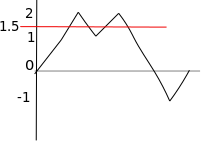
\includegraphics[]{count_2.png}
\end{document}